\documentclass[]{article}
\usepackage{lmodern}
\usepackage{amssymb,amsmath}
\usepackage{ifxetex,ifluatex}
\usepackage{fixltx2e} % provides \textsubscript
\ifnum 0\ifxetex 1\fi\ifluatex 1\fi=0 % if pdftex
  \usepackage[T1]{fontenc}
  \usepackage[utf8]{inputenc}
\else % if luatex or xelatex
  \ifxetex
    \usepackage{mathspec}
  \else
    \usepackage{fontspec}
  \fi
  \defaultfontfeatures{Ligatures=TeX,Scale=MatchLowercase}
\fi
% use upquote if available, for straight quotes in verbatim environments
\IfFileExists{upquote.sty}{\usepackage{upquote}}{}
% use microtype if available
\IfFileExists{microtype.sty}{%
\usepackage{microtype}
\UseMicrotypeSet[protrusion]{basicmath} % disable protrusion for tt fonts
}{}
\usepackage[margin=1in]{geometry}
\usepackage{hyperref}
\hypersetup{unicode=true,
            pdftitle={Data Visualization},
            pdfauthor={Jennifer Brazeal},
            pdfborder={0 0 0},
            breaklinks=true}
\urlstyle{same}  % don't use monospace font for urls
\usepackage{color}
\usepackage{fancyvrb}
\newcommand{\VerbBar}{|}
\newcommand{\VERB}{\Verb[commandchars=\\\{\}]}
\DefineVerbatimEnvironment{Highlighting}{Verbatim}{commandchars=\\\{\}}
% Add ',fontsize=\small' for more characters per line
\usepackage{framed}
\definecolor{shadecolor}{RGB}{248,248,248}
\newenvironment{Shaded}{\begin{snugshade}}{\end{snugshade}}
\newcommand{\AlertTok}[1]{\textcolor[rgb]{0.94,0.16,0.16}{#1}}
\newcommand{\AnnotationTok}[1]{\textcolor[rgb]{0.56,0.35,0.01}{\textbf{\textit{#1}}}}
\newcommand{\AttributeTok}[1]{\textcolor[rgb]{0.77,0.63,0.00}{#1}}
\newcommand{\BaseNTok}[1]{\textcolor[rgb]{0.00,0.00,0.81}{#1}}
\newcommand{\BuiltInTok}[1]{#1}
\newcommand{\CharTok}[1]{\textcolor[rgb]{0.31,0.60,0.02}{#1}}
\newcommand{\CommentTok}[1]{\textcolor[rgb]{0.56,0.35,0.01}{\textit{#1}}}
\newcommand{\CommentVarTok}[1]{\textcolor[rgb]{0.56,0.35,0.01}{\textbf{\textit{#1}}}}
\newcommand{\ConstantTok}[1]{\textcolor[rgb]{0.00,0.00,0.00}{#1}}
\newcommand{\ControlFlowTok}[1]{\textcolor[rgb]{0.13,0.29,0.53}{\textbf{#1}}}
\newcommand{\DataTypeTok}[1]{\textcolor[rgb]{0.13,0.29,0.53}{#1}}
\newcommand{\DecValTok}[1]{\textcolor[rgb]{0.00,0.00,0.81}{#1}}
\newcommand{\DocumentationTok}[1]{\textcolor[rgb]{0.56,0.35,0.01}{\textbf{\textit{#1}}}}
\newcommand{\ErrorTok}[1]{\textcolor[rgb]{0.64,0.00,0.00}{\textbf{#1}}}
\newcommand{\ExtensionTok}[1]{#1}
\newcommand{\FloatTok}[1]{\textcolor[rgb]{0.00,0.00,0.81}{#1}}
\newcommand{\FunctionTok}[1]{\textcolor[rgb]{0.00,0.00,0.00}{#1}}
\newcommand{\ImportTok}[1]{#1}
\newcommand{\InformationTok}[1]{\textcolor[rgb]{0.56,0.35,0.01}{\textbf{\textit{#1}}}}
\newcommand{\KeywordTok}[1]{\textcolor[rgb]{0.13,0.29,0.53}{\textbf{#1}}}
\newcommand{\NormalTok}[1]{#1}
\newcommand{\OperatorTok}[1]{\textcolor[rgb]{0.81,0.36,0.00}{\textbf{#1}}}
\newcommand{\OtherTok}[1]{\textcolor[rgb]{0.56,0.35,0.01}{#1}}
\newcommand{\PreprocessorTok}[1]{\textcolor[rgb]{0.56,0.35,0.01}{\textit{#1}}}
\newcommand{\RegionMarkerTok}[1]{#1}
\newcommand{\SpecialCharTok}[1]{\textcolor[rgb]{0.00,0.00,0.00}{#1}}
\newcommand{\SpecialStringTok}[1]{\textcolor[rgb]{0.31,0.60,0.02}{#1}}
\newcommand{\StringTok}[1]{\textcolor[rgb]{0.31,0.60,0.02}{#1}}
\newcommand{\VariableTok}[1]{\textcolor[rgb]{0.00,0.00,0.00}{#1}}
\newcommand{\VerbatimStringTok}[1]{\textcolor[rgb]{0.31,0.60,0.02}{#1}}
\newcommand{\WarningTok}[1]{\textcolor[rgb]{0.56,0.35,0.01}{\textbf{\textit{#1}}}}
\usepackage{graphicx,grffile}
\makeatletter
\def\maxwidth{\ifdim\Gin@nat@width>\linewidth\linewidth\else\Gin@nat@width\fi}
\def\maxheight{\ifdim\Gin@nat@height>\textheight\textheight\else\Gin@nat@height\fi}
\makeatother
% Scale images if necessary, so that they will not overflow the page
% margins by default, and it is still possible to overwrite the defaults
% using explicit options in \includegraphics[width, height, ...]{}
\setkeys{Gin}{width=\maxwidth,height=\maxheight,keepaspectratio}
\IfFileExists{parskip.sty}{%
\usepackage{parskip}
}{% else
\setlength{\parindent}{0pt}
\setlength{\parskip}{6pt plus 2pt minus 1pt}
}
\setlength{\emergencystretch}{3em}  % prevent overfull lines
\providecommand{\tightlist}{%
  \setlength{\itemsep}{0pt}\setlength{\parskip}{0pt}}
\setcounter{secnumdepth}{0}
% Redefines (sub)paragraphs to behave more like sections
\ifx\paragraph\undefined\else
\let\oldparagraph\paragraph
\renewcommand{\paragraph}[1]{\oldparagraph{#1}\mbox{}}
\fi
\ifx\subparagraph\undefined\else
\let\oldsubparagraph\subparagraph
\renewcommand{\subparagraph}[1]{\oldsubparagraph{#1}\mbox{}}
\fi

%%% Use protect on footnotes to avoid problems with footnotes in titles
\let\rmarkdownfootnote\footnote%
\def\footnote{\protect\rmarkdownfootnote}

%%% Change title format to be more compact
\usepackage{titling}

% Create subtitle command for use in maketitle
\providecommand{\subtitle}[1]{
  \posttitle{
    \begin{center}\large#1\end{center}
    }
}

\setlength{\droptitle}{-2em}

  \title{Data Visualization}
    \pretitle{\vspace{\droptitle}\centering\huge}
  \posttitle{\par}
    \author{Jennifer Brazeal}
    \preauthor{\centering\large\emph}
  \postauthor{\par}
      \predate{\centering\large\emph}
  \postdate{\par}
    \date{9/5/19}


\begin{document}
\maketitle

Data visualization is an important tool for both data exploration and
for communicating your results effectively to peers and to the public.
Today we will show you some of the things you can do using base R
plotting functions to explore the CO2 dataset. A package called ggplot2,
part of a larger set of packages known as the ``tidyverse,'' is popular
for data visualization. We will introduce you to ggplot2 on the final
day of class, but we first want to give you a good grounding in base R
plotting functions.

Before we get started, let's save the CO2 data again from the internal
\texttt{datasets} package as an object in our workspace. This dataset
contains observations of CO2 uptake by plants originating from different
locations (Quebec and Mississippi) and under different temperature
treatments (chilled and not chilled) across different fixed ambient CO2
concentrations.

\begin{Shaded}
\begin{Highlighting}[]
\NormalTok{?CO2}
\end{Highlighting}
\end{Shaded}

\begin{verbatim}
## starting httpd help server ... done
\end{verbatim}

\begin{Shaded}
\begin{Highlighting}[]
\NormalTok{CO2 <-}\StringTok{ }\NormalTok{datasets}\OperatorTok{::}\NormalTok{CO2}
\end{Highlighting}
\end{Shaded}

The head() function lets us take a quick look at the data - three
columns of character vectors and two numeric columns:

\begin{Shaded}
\begin{Highlighting}[]
\KeywordTok{head}\NormalTok{(CO2)}
\end{Highlighting}
\end{Shaded}

\begin{verbatim}
##   Plant   Type  Treatment conc uptake
## 1   Qn1 Quebec nonchilled   95   16.0
## 2   Qn1 Quebec nonchilled  175   30.4
## 3   Qn1 Quebec nonchilled  250   34.8
## 4   Qn1 Quebec nonchilled  350   37.2
## 5   Qn1 Quebec nonchilled  500   35.3
## 6   Qn1 Quebec nonchilled  675   39.2
\end{verbatim}

str() shows us more specific information about the structure of the
data:

\begin{Shaded}
\begin{Highlighting}[]
\KeywordTok{str}\NormalTok{(CO2)}
\end{Highlighting}
\end{Shaded}

\begin{verbatim}
## Classes 'nfnGroupedData', 'nfGroupedData', 'groupedData' and 'data.frame':   84 obs. of  5 variables:
##  $ Plant    : Ord.factor w/ 12 levels "Qn1"<"Qn2"<"Qn3"<..: 1 1 1 1 1 1 1 2 2 2 ...
##  $ Type     : Factor w/ 2 levels "Quebec","Mississippi": 1 1 1 1 1 1 1 1 1 1 ...
##  $ Treatment: Factor w/ 2 levels "nonchilled","chilled": 1 1 1 1 1 1 1 1 1 1 ...
##  $ conc     : num  95 175 250 350 500 675 1000 95 175 250 ...
##  $ uptake   : num  16 30.4 34.8 37.2 35.3 39.2 39.7 13.6 27.3 37.1 ...
##  - attr(*, "formula")=Class 'formula'  language uptake ~ conc | Plant
##   .. ..- attr(*, ".Environment")=<environment: R_EmptyEnv> 
##  - attr(*, "outer")=Class 'formula'  language ~Treatment * Type
##   .. ..- attr(*, ".Environment")=<environment: R_EmptyEnv> 
##  - attr(*, "labels")=List of 2
##   ..$ x: chr "Ambient carbon dioxide concentration"
##   ..$ y: chr "CO2 uptake rate"
##  - attr(*, "units")=List of 2
##   ..$ x: chr "(uL/L)"
##   ..$ y: chr "(umol/m^2 s)"
\end{verbatim}

Questions: what units are the uptake rate in?

\hypertarget{different-plot-types}{%
\subsection{Different Plot Types}\label{different-plot-types}}

\hypertarget{plotting-one-continuous-variable}{%
\subsubsection{Plotting one continuous
variable}\label{plotting-one-continuous-variable}}

\hypertarget{histograms---groups-the-data-into-bins-default-or-custom-defined-spanning-the-range-of-the-data-and-displays-the-frequency-of-each-bin.}{%
\paragraph{\texorpdfstring{\emph{Histograms} - groups the data into bins
(default or custom defined) spanning the range of the data, and displays
the frequency of each
bin.}{Histograms - groups the data into bins (default or custom defined) spanning the range of the data, and displays the frequency of each bin.}}\label{histograms---groups-the-data-into-bins-default-or-custom-defined-spanning-the-range-of-the-data-and-displays-the-frequency-of-each-bin.}}

\begin{Shaded}
\begin{Highlighting}[]
\NormalTok{?hist}
\end{Highlighting}
\end{Shaded}

Examples:

\begin{Shaded}
\begin{Highlighting}[]
\KeywordTok{hist}\NormalTok{(CO2}\OperatorTok{$}\NormalTok{uptake)}
\end{Highlighting}
\end{Shaded}

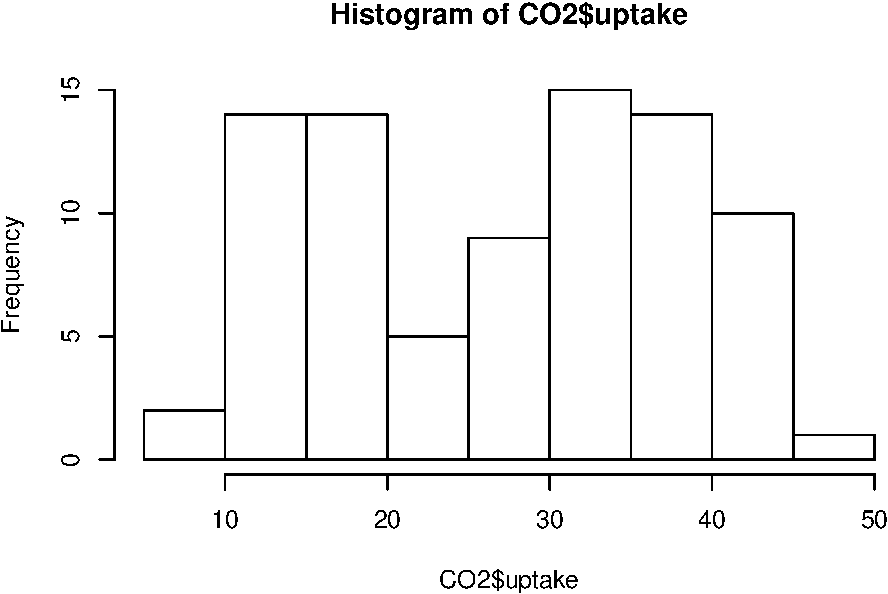
\includegraphics{Plotting_JB_files/figure-latex/unnamed-chunk-5-1.pdf}

\hypertarget{density-plots---smooths-univariate-data-into-a-continuous-density-along-its-range.}{%
\paragraph{Density plots - Smooths univariate data into a continuous
density along its
range.}\label{density-plots---smooths-univariate-data-into-a-continuous-density-along-its-range.}}

\begin{Shaded}
\begin{Highlighting}[]
\NormalTok{?density }\CommentTok{# Combine with plot() to vizualize; i.e. plot(density(x))}
\end{Highlighting}
\end{Shaded}

Example:

\begin{Shaded}
\begin{Highlighting}[]
\KeywordTok{density}\NormalTok{(CO2}\OperatorTok{$}\NormalTok{uptake)}
\end{Highlighting}
\end{Shaded}

\begin{verbatim}
## 
## Call:
##  density.default(x = CO2$uptake)
## 
## Data: CO2$uptake (84 obs.);  Bandwidth 'bw' = 4.012
## 
##        x                y            
##  Min.   :-4.337   Min.   :2.286e-05  
##  1st Qu.:11.132   1st Qu.:2.863e-03  
##  Median :26.600   Median :2.125e-02  
##  Mean   :26.600   Mean   :1.615e-02  
##  3rd Qu.:42.068   3rd Qu.:2.649e-02  
##  Max.   :57.537   Max.   :3.095e-02
\end{verbatim}

\begin{Shaded}
\begin{Highlighting}[]
\KeywordTok{plot}\NormalTok{(}\KeywordTok{density}\NormalTok{(CO2}\OperatorTok{$}\NormalTok{uptake))}
\end{Highlighting}
\end{Shaded}

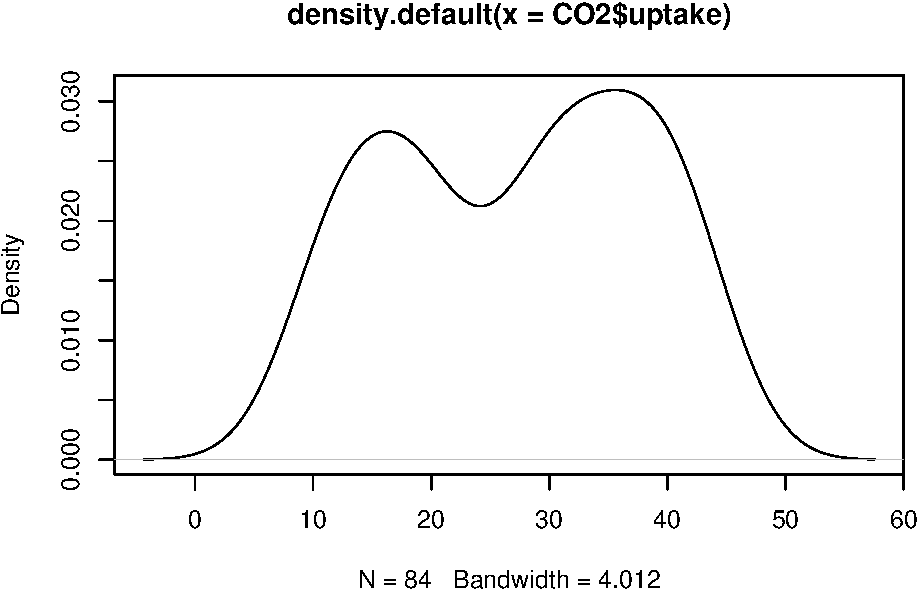
\includegraphics{Plotting_JB_files/figure-latex/unnamed-chunk-7-1.pdf}

\hypertarget{dotcharts---displays-all-point-values-along-one-dimension.-the-x-axis-corresponds-to-the-value-you-are-plotting-while-the-y-axis-separates-out-the-different-data-points}{%
\paragraph{Dotcharts - Displays all point values along one dimension.
The X-axis corresponds to the value you are plotting, while the Y-axis
separates out the different data
points}\label{dotcharts---displays-all-point-values-along-one-dimension.-the-x-axis-corresponds-to-the-value-you-are-plotting-while-the-y-axis-separates-out-the-different-data-points}}

\begin{Shaded}
\begin{Highlighting}[]
\NormalTok{?dotchart}
\end{Highlighting}
\end{Shaded}

Examples:

\begin{Shaded}
\begin{Highlighting}[]
\KeywordTok{dotchart}\NormalTok{(CO2}\OperatorTok{$}\NormalTok{uptake) }\CommentTok{# separate out data by plant origin}
\end{Highlighting}
\end{Shaded}

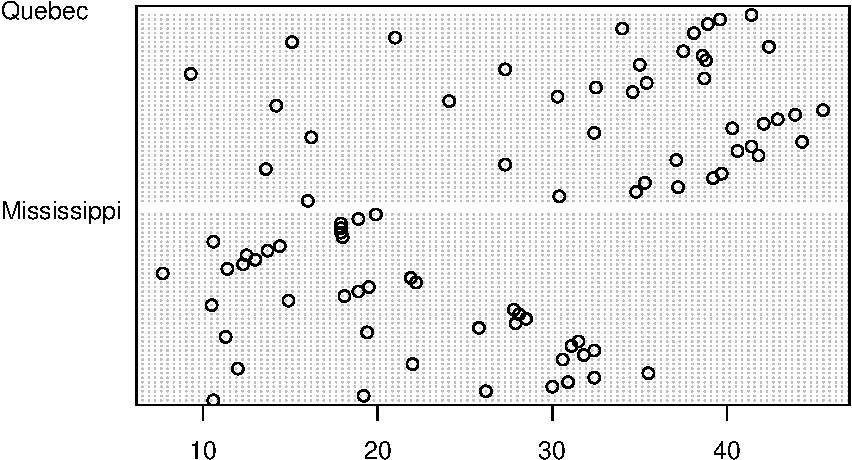
\includegraphics{Plotting_JB_files/figure-latex/unnamed-chunk-9-1.pdf}

Note, you can also specify a grouping factor to divide the points and
visually compare by group

\begin{Shaded}
\begin{Highlighting}[]
\KeywordTok{dotchart}\NormalTok{(CO2}\OperatorTok{$}\NormalTok{uptake, }\DataTypeTok{groups =}\NormalTok{ CO2}\OperatorTok{$}\NormalTok{Type) }\CommentTok{# separate out data by plant origin}
\end{Highlighting}
\end{Shaded}

\includegraphics{Plotting_JB_files/figure-latex/unnamed-chunk-10-1.pdf}

\begin{Shaded}
\begin{Highlighting}[]
\KeywordTok{dotchart}\NormalTok{(CO2}\OperatorTok{$}\NormalTok{uptake, }\DataTypeTok{groups =}\NormalTok{ CO2}\OperatorTok{$}\NormalTok{Treatment) }\CommentTok{# And do the same for the different treatments (chilled vs. non-chilled)}
\end{Highlighting}
\end{Shaded}

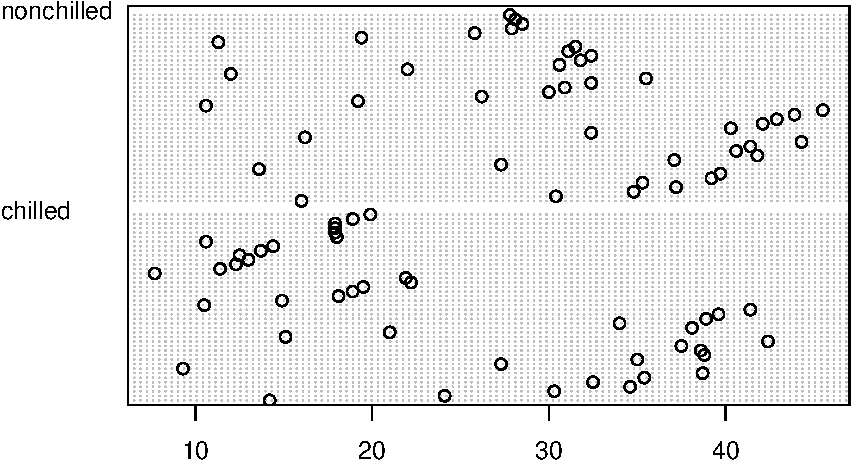
\includegraphics{Plotting_JB_files/figure-latex/unnamed-chunk-10-2.pdf}

You might also be interested in what the data looks like for different
plant origins when divided up by treatment. You can use the ``col''
argument to color by a factor level:

\begin{Shaded}
\begin{Highlighting}[]
\KeywordTok{dotchart}\NormalTok{(CO2}\OperatorTok{$}\NormalTok{uptake, }\DataTypeTok{groups =}\NormalTok{ CO2}\OperatorTok{$}\NormalTok{Treatment, }\DataTypeTok{col =}\NormalTok{ CO2}\OperatorTok{$}\NormalTok{Type) }
\end{Highlighting}
\end{Shaded}

\includegraphics{Plotting_JB_files/figure-latex/unnamed-chunk-11-1.pdf}

But, which color corresponds to Quebec, and which to Mississippi? You
can add a legend using the same factor levels to make this clear:

\begin{Shaded}
\begin{Highlighting}[]
\KeywordTok{dotchart}\NormalTok{(CO2}\OperatorTok{$}\NormalTok{uptake, }
         \DataTypeTok{groups =}\NormalTok{ CO2}\OperatorTok{$}\NormalTok{Treatment, }
         \DataTypeTok{col =}\NormalTok{ CO2}\OperatorTok{$}\NormalTok{Type,}
         \DataTypeTok{pch =} \DecValTok{19}\NormalTok{) }\CommentTok{# Set the marker type so it is the same in the plot and in the legend.  }

\KeywordTok{legend}\NormalTok{(}\DataTypeTok{x =} \StringTok{"topright"}\NormalTok{,}
       \DataTypeTok{legend =} \KeywordTok{levels}\NormalTok{(CO2}\OperatorTok{$}\NormalTok{Type), }\CommentTok{# Using levels() here pulls out the unique factor levels for your legend text, in the same order that it gets colored above.}
       \DataTypeTok{col =} \DecValTok{1}\OperatorTok{:}\KeywordTok{length}\NormalTok{(CO2}\OperatorTok{$}\NormalTok{Type), }\CommentTok{# For coloring the marker, you want a series of numbers that are the same length as the items in the legend.  This pulls out that number of colors from the current palette you have set in R (more on this later)}
       \DataTypeTok{pch =} \DecValTok{19}\NormalTok{)}
\end{Highlighting}
\end{Shaded}

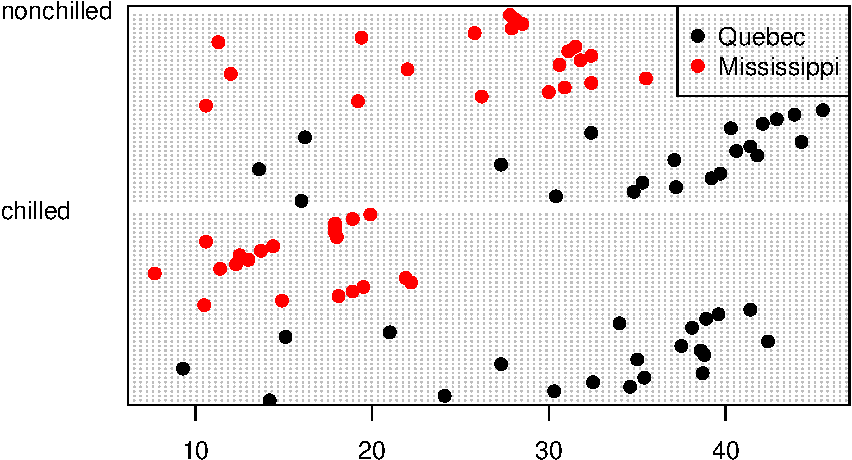
\includegraphics{Plotting_JB_files/figure-latex/unnamed-chunk-12-1.pdf}

Question: so far in our visual data exploration, what have you noticed
about CO2 uptake by plant country origin? What about by treatment?

\hypertarget{plotting-two-variables}{%
\subsubsection{Plotting two variables}\label{plotting-two-variables}}

\hypertarget{scatterplots-2-continuous-variables}{%
\paragraph{Scatterplots: 2 continuous
variables}\label{scatterplots-2-continuous-variables}}

We can use a scatterplot to look at how uptake rate changes with ambient
CO2 concentration:

\begin{Shaded}
\begin{Highlighting}[]
\KeywordTok{plot}\NormalTok{(}\DataTypeTok{x =}\NormalTok{ CO2}\OperatorTok{$}\NormalTok{conc, }
     \DataTypeTok{y =}\NormalTok{ CO2}\OperatorTok{$}\NormalTok{uptake)}
\end{Highlighting}
\end{Shaded}

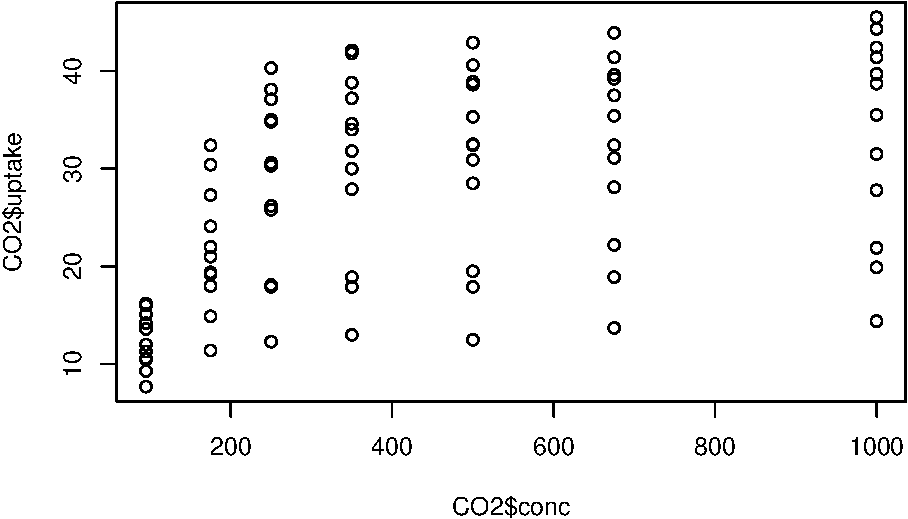
\includegraphics{Plotting_JB_files/figure-latex/unnamed-chunk-13-1.pdf}

\begin{Shaded}
\begin{Highlighting}[]
\CommentTok{# an alternative way of writing the above is:}

\KeywordTok{plot}\NormalTok{(}\DataTypeTok{formula =}\NormalTok{ uptake }\OperatorTok{~}\StringTok{ }\NormalTok{conc, }
     \DataTypeTok{data =}\NormalTok{ CO2)}
\end{Highlighting}
\end{Shaded}

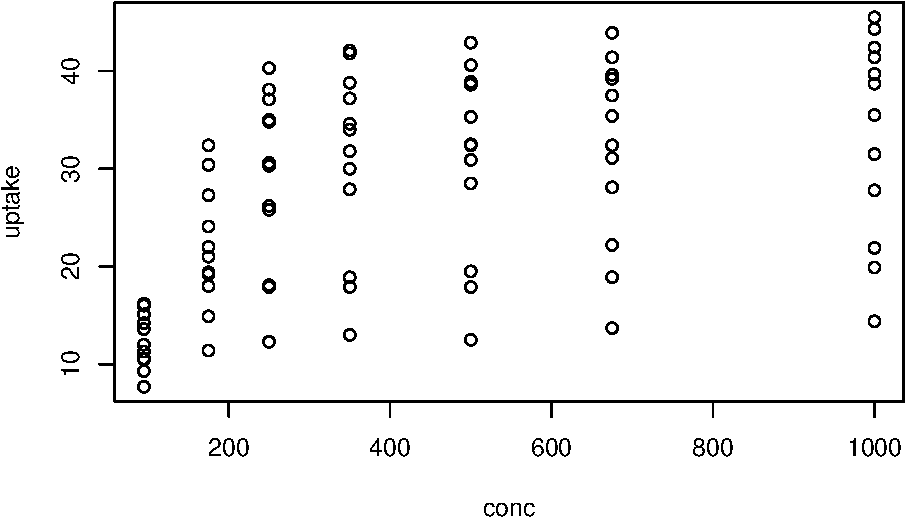
\includegraphics{Plotting_JB_files/figure-latex/unnamed-chunk-13-2.pdf}
Tip: the tilde signifies that the left side variable is a response
(i.e., the ``y'' variable) to the right side variable (i.e., the ``x''
variable). The same notation is used in statistical modeling, which you
will see tomorrow.

\hypertarget{box-plots---groups-the-data-along-discrete-factors-and-display-the-median-interquartile-range-whiskers-and-outliers}{%
\subsubsection{Box plots - Groups the data along discrete factors, and
display the median, interquartile range (whiskers), and
outliers}\label{box-plots---groups-the-data-along-discrete-factors-and-display-the-median-interquartile-range-whiskers-and-outliers}}

You can do this 2 ways: specify a categorical (factor level) X variable
in plot(), which will automatically produce a boxplot, or use the
boxplot() function directly.

\begin{Shaded}
\begin{Highlighting}[]
\KeywordTok{plot}\NormalTok{(}\DataTypeTok{x =}\NormalTok{ CO2}\OperatorTok{$}\NormalTok{Treatment, }
     \DataTypeTok{y =}\NormalTok{ CO2}\OperatorTok{$}\NormalTok{uptake) }
\end{Highlighting}
\end{Shaded}

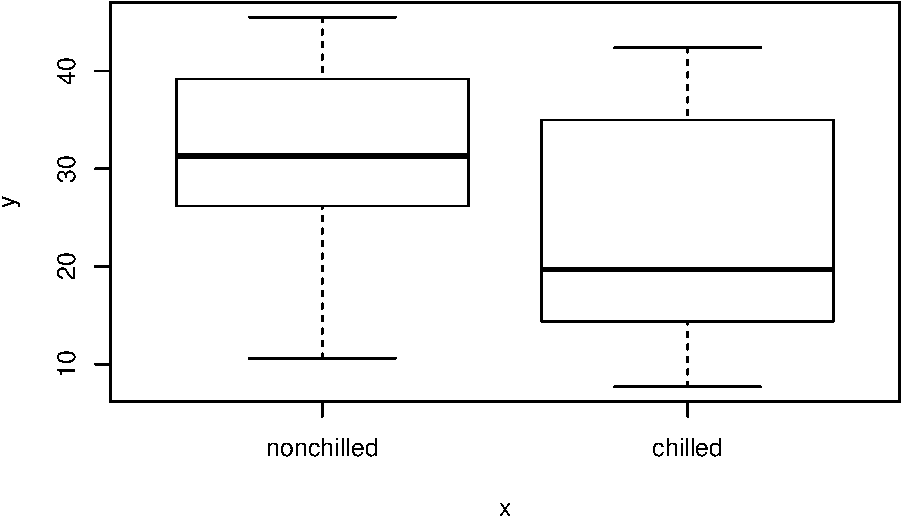
\includegraphics{Plotting_JB_files/figure-latex/unnamed-chunk-14-1.pdf}

Before using the boxplot function, let's take a quick look at its help
file to understand the different arguments:

\begin{Shaded}
\begin{Highlighting}[]
\NormalTok{?boxplot}
\KeywordTok{boxplot}\NormalTok{(}\DataTypeTok{formula =}\NormalTok{ uptake }\OperatorTok{~}\StringTok{ }\NormalTok{Treatment, }
        \DataTypeTok{data =}\NormalTok{ CO2)}
\end{Highlighting}
\end{Shaded}

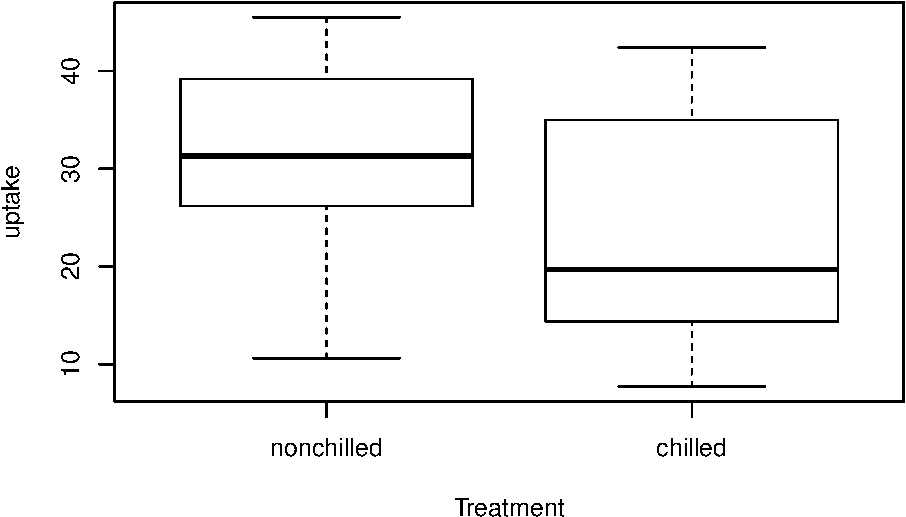
\includegraphics{Plotting_JB_files/figure-latex/unnamed-chunk-15-1.pdf}

\hypertarget{characteristics-of-good-data-plots}{%
\section{Characteristics of good data
plots:}\label{characteristics-of-good-data-plots}}

\begin{itemize}
\tightlist
\item
  A purpose, clearly defined set of variables, and a message to convey.
\item
  Succinct and uncluttered so as to allow easy interpretation of the
  purpose.
\item
  Comprehensive, representing the data accurately and fairly.
\end{itemize}

Let's now take a closer look at the different plot types using our CO2
dataset to ask biological questions and explore relationships.

\hypertarget{scatterplots}{%
\section{Scatterplots}\label{scatterplots}}

changing ambient CO2 should affect CO2 uptake - we predict that less CO2
available might result in a slower uptake rate. Can we see this in the
data?

We are interested in two numeric variables, so let's look at a
scatterplot of our data:

\begin{Shaded}
\begin{Highlighting}[]
\KeywordTok{class}\NormalTok{(CO2}\OperatorTok{$}\NormalTok{conc)}
\end{Highlighting}
\end{Shaded}

\begin{verbatim}
## [1] "numeric"
\end{verbatim}

\begin{Shaded}
\begin{Highlighting}[]
\KeywordTok{class}\NormalTok{(CO2}\OperatorTok{$}\NormalTok{uptake)}
\end{Highlighting}
\end{Shaded}

\begin{verbatim}
## [1] "numeric"
\end{verbatim}

\begin{Shaded}
\begin{Highlighting}[]
\KeywordTok{plot}\NormalTok{(}\DataTypeTok{x =}\NormalTok{ CO2}\OperatorTok{$}\NormalTok{conc, }\DataTypeTok{y =}\NormalTok{ CO2}\OperatorTok{$}\NormalTok{uptake)}
\end{Highlighting}
\end{Shaded}

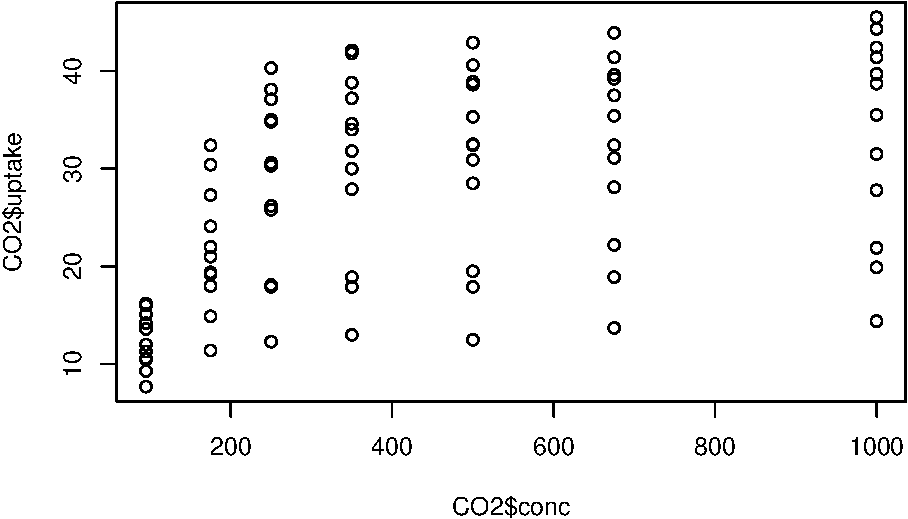
\includegraphics{Plotting_JB_files/figure-latex/unnamed-chunk-16-1.pdf}

The ambient concentration variable was a fixed variable, so we have
several observations within single values, which is why the plot looks
discontinuous. We might also be interested in the averages of CO2 uptake
within each ambient CO2 concentration:

First let's get the means:

\begin{Shaded}
\begin{Highlighting}[]
\NormalTok{(uptakeMeans <-}\StringTok{ }\KeywordTok{aggregate}\NormalTok{(uptake }\OperatorTok{~}\StringTok{ }\NormalTok{conc, }\DataTypeTok{data =}\NormalTok{ CO2, }\DataTypeTok{FUN =}\NormalTok{ mean))}
\end{Highlighting}
\end{Shaded}

\begin{verbatim}
##   conc   uptake
## 1   95 12.25833
## 2  175 22.28333
## 3  250 28.87500
## 4  350 30.66667
## 5  500 30.87500
## 6  675 31.95000
## 7 1000 33.58333
\end{verbatim}

\begin{Shaded}
\begin{Highlighting}[]
\KeywordTok{names}\NormalTok{(uptakeMeans) <-}\StringTok{ }\KeywordTok{c}\NormalTok{(}\StringTok{"conc"}\NormalTok{, }\StringTok{"mean"}\NormalTok{)}
\end{Highlighting}
\end{Shaded}

We could plot the means, then add the original data points to see the
total sample spread of data around the mean. (Honestly, this is just to
illustrate the ability to add things to a plot with functions such as
points and lines)

\begin{Shaded}
\begin{Highlighting}[]
\KeywordTok{plot}\NormalTok{(mean }\OperatorTok{~}\StringTok{ }\NormalTok{conc, }
     \DataTypeTok{data =}\NormalTok{ uptakeMeans,}
     \DataTypeTok{pch =} \DecValTok{19}\NormalTok{, }\CommentTok{# set the pch to a solid dot to differentiation the mean from the rest of the data}
     \DataTypeTok{ylim =} \KeywordTok{c}\NormalTok{(}\KeywordTok{min}\NormalTok{(CO2}\OperatorTok{$}\NormalTok{uptake), }\KeywordTok{max}\NormalTok{(CO2}\OperatorTok{$}\NormalTok{uptake))) }\CommentTok{# Change the y limits to accomodate the total data spread.}
     
\KeywordTok{points}\NormalTok{(CO2}\OperatorTok{$}\NormalTok{uptake }\OperatorTok{~}\StringTok{ }\NormalTok{CO2}\OperatorTok{$}\NormalTok{conc, }\DataTypeTok{col =} \StringTok{"grey"}\NormalTok{)}
\end{Highlighting}
\end{Shaded}

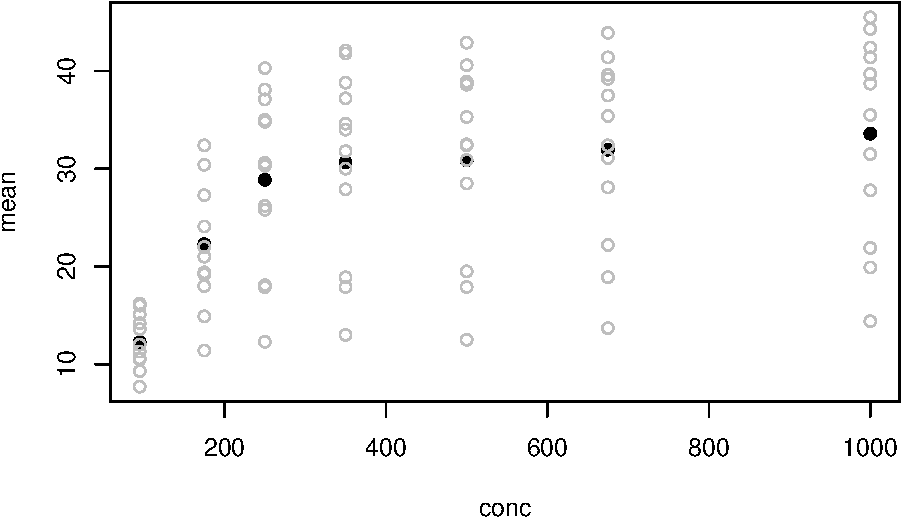
\includegraphics{Plotting_JB_files/figure-latex/unnamed-chunk-18-1.pdf}

For fun, lets add a line across the means too.

\begin{Shaded}
\begin{Highlighting}[]
\KeywordTok{plot}\NormalTok{(mean }\OperatorTok{~}\StringTok{ }\NormalTok{conc, }
     \DataTypeTok{data =}\NormalTok{ uptakeMeans,}
     \DataTypeTok{pch =} \DecValTok{19}\NormalTok{, }\CommentTok{# set the pch to a solid dot to differentiation the mean from the rest of the data}
     \DataTypeTok{ylim =} \KeywordTok{c}\NormalTok{(}\KeywordTok{min}\NormalTok{(CO2}\OperatorTok{$}\NormalTok{uptake), }\KeywordTok{max}\NormalTok{(CO2}\OperatorTok{$}\NormalTok{uptake))) }\CommentTok{# Change the y limits again to accomodate the total data spread.}
     
\KeywordTok{points}\NormalTok{(CO2}\OperatorTok{$}\NormalTok{uptake }\OperatorTok{~}\StringTok{ }\NormalTok{CO2}\OperatorTok{$}\NormalTok{conc, }\DataTypeTok{col =} \StringTok{"grey"}\NormalTok{)}

\KeywordTok{lines}\NormalTok{(mean }\OperatorTok{~}\StringTok{ }\NormalTok{conc, }
      \DataTypeTok{data =}\NormalTok{ uptakeMeans)}
\end{Highlighting}
\end{Shaded}

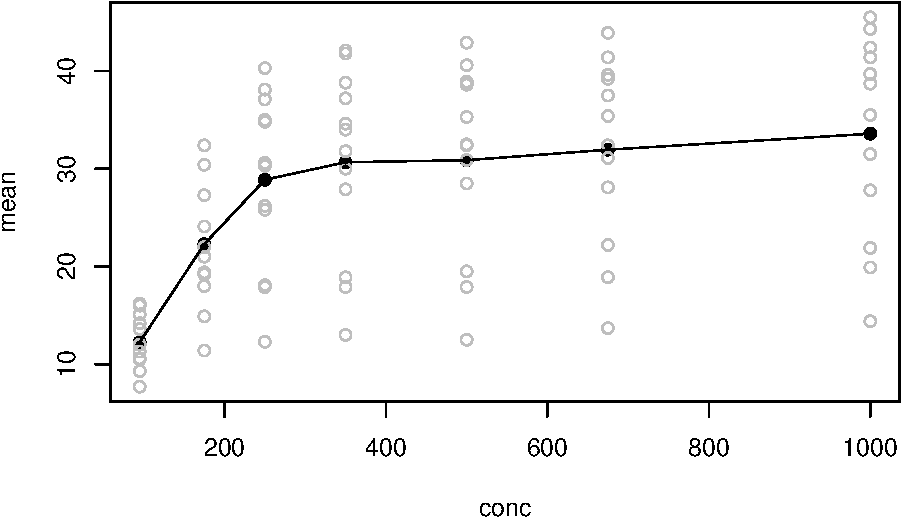
\includegraphics{Plotting_JB_files/figure-latex/unnamed-chunk-19-1.pdf}

But instead of plotting all the data with the means, it's usually a good
idea to plot some kind of error bar around each mean to succinctly show
variation around the average. Different error bars serve different
purposes. Since we are just interested in looking at the spread of our
uptake data at each ambient CO2 concentration, we will add standard
deviation bars.

\begin{Shaded}
\begin{Highlighting}[]
\CommentTok{# First, let's get the sds, aggregated by concentration. }
\NormalTok{(uptakeSD <-}\StringTok{ }\KeywordTok{aggregate}\NormalTok{(uptake }\OperatorTok{~}\StringTok{ }\NormalTok{conc, }\DataTypeTok{data =}\NormalTok{ CO2, }\DataTypeTok{FUN =}\NormalTok{ sd))}
\end{Highlighting}
\end{Shaded}

\begin{verbatim}
##   conc    uptake
## 1   95  2.735111
## 2  175  6.271992
## 3  250  8.988895
## 4  350  9.596527
## 5  500  9.671056
## 6  675  9.534960
## 7 1000 10.411867
\end{verbatim}

\begin{Shaded}
\begin{Highlighting}[]
\KeywordTok{names}\NormalTok{(uptakeSD) <-}\StringTok{ }\KeywordTok{c}\NormalTok{(}\StringTok{"conc"}\NormalTok{, }\StringTok{"sd"}\NormalTok{)}

\KeywordTok{plot}\NormalTok{(mean }\OperatorTok{~}\StringTok{ }\NormalTok{conc, }
     \DataTypeTok{data =}\NormalTok{ uptakeMeans,}
     \DataTypeTok{ylim =} \KeywordTok{c}\NormalTok{(}\DecValTok{0}\NormalTok{, }\DecValTok{45}\NormalTok{)) }\CommentTok{# we again expand the default Y-axis limits to accomodate the sd bars. I chose these values throuh quivk plotting trial and error, but you could also add/substract the sd from the min and max uptake values to know where your bounds should be at minimum. }

\CommentTok{# like lines() and points(), arrows() adds arrows to an already existing plot. It literally plots arrows, but we set the length of the arrowheads to be 0 for a clean bar without caps.  You could add the arguments (angle = 90, length = XX, code = 3) to draw more typical error bar caps of a given length instead. }

\KeywordTok{arrows}\NormalTok{(}\DataTypeTok{x0 =}\NormalTok{ uptakeMeans}\OperatorTok{$}\NormalTok{conc, }
       \DataTypeTok{y0 =}\NormalTok{ uptakeMeans}\OperatorTok{$}\NormalTok{mean }\OperatorTok{-}\StringTok{ }\NormalTok{uptakeSD}\OperatorTok{$}\NormalTok{sd,}
       \DataTypeTok{y1 =}\NormalTok{ uptakeMeans}\OperatorTok{$}\NormalTok{mean }\OperatorTok{+}\StringTok{ }\NormalTok{uptakeSD}\OperatorTok{$}\NormalTok{sd,}
       \DataTypeTok{length =} \DecValTok{0}\NormalTok{)}
\end{Highlighting}
\end{Shaded}

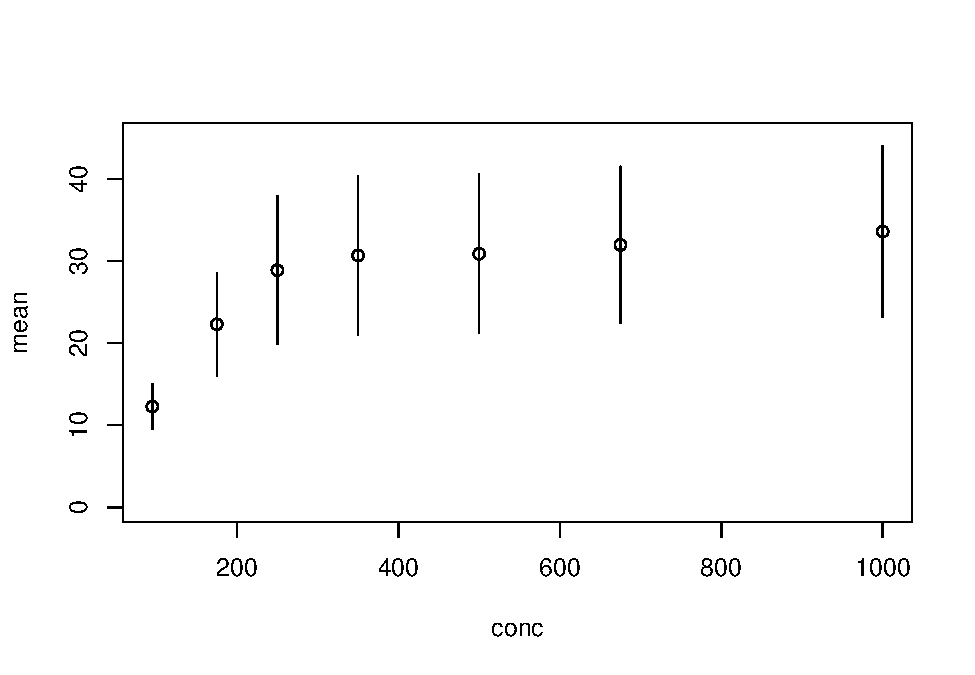
\includegraphics{Plotting_JB_files/figure-latex/unnamed-chunk-20-1.pdf}

\begin{Shaded}
\begin{Highlighting}[]
\CommentTok{# x0, x1 and y0, y1 are where you draw the start (0) and end (1) of the bars. x1 and y1 default to x0 and y0 unless you specify otherwise.  Note, you cannot specify only x0, and y0, as then you will be drawing points.  }
\end{Highlighting}
\end{Shaded}

You can also plot this directly as a line plot by setting the ``type''
argument to ``l'' for lines or ``b'' for both points and lines. It
defaults to ``p'' for points.

\begin{Shaded}
\begin{Highlighting}[]
\KeywordTok{plot}\NormalTok{(mean }\OperatorTok{~}\StringTok{ }\NormalTok{conc, }
     \DataTypeTok{data =}\NormalTok{ uptakeMeans,}
     \DataTypeTok{ylim =} \KeywordTok{c}\NormalTok{(}\DecValTok{0}\NormalTok{, }\DecValTok{45}\NormalTok{), }
     \DataTypeTok{type =} \StringTok{"b"}\NormalTok{)}
\KeywordTok{arrows}\NormalTok{(}\DataTypeTok{x0 =}\NormalTok{ uptakeMeans}\OperatorTok{$}\NormalTok{conc, }
       \DataTypeTok{y0 =}\NormalTok{ uptakeMeans}\OperatorTok{$}\NormalTok{mean }\OperatorTok{-}\StringTok{ }\NormalTok{uptakeSD}\OperatorTok{$}\NormalTok{sd,}
       \DataTypeTok{y1 =}\NormalTok{ uptakeMeans}\OperatorTok{$}\NormalTok{mean }\OperatorTok{+}\StringTok{ }\NormalTok{uptakeSD}\OperatorTok{$}\NormalTok{sd,}
       \DataTypeTok{angle =} \DecValTok{90}\NormalTok{,}
       \DataTypeTok{code =} \DecValTok{3}\NormalTok{,}
       \DataTypeTok{length =} \FloatTok{0.1}\NormalTok{) }
\end{Highlighting}
\end{Shaded}

\includegraphics{Plotting_JB_files/figure-latex/unnamed-chunk-21-1.pdf}
Commentary: There's an increase in uptake as the concentration gradient
increases, but it doesn't really increase much after
\textasciitilde{}250 uL/L. It may imply that CO2 concentration is only a
limiting factor at very low levels and does not drive uptake at higher
concentrations.

\hypertarget{lets-look-at-some-ways-we-can-make-our-plots-look-a-little-better-and-be-more-easily-interpreted.}{%
\paragraph{Let's look at some ways we can make our plots look a little
better and be more easily
interpreted.}\label{lets-look-at-some-ways-we-can-make-our-plots-look-a-little-better-and-be-more-easily-interpreted.}}

First, we can add some labels and a title:

\begin{Shaded}
\begin{Highlighting}[]
\KeywordTok{plot}\NormalTok{(}\DataTypeTok{x =}\NormalTok{ CO2}\OperatorTok{$}\NormalTok{conc, }\DataTypeTok{y =}\NormalTok{ CO2}\OperatorTok{$}\NormalTok{uptake, }
     \DataTypeTok{xlab =} \StringTok{'CO2 Conc. uL/L'}\NormalTok{, }
     \DataTypeTok{ylab =} \StringTok{'CO2 Uptake (umol/m^2 sec)'}\NormalTok{, }
     \DataTypeTok{main =} \StringTok{'CO2 Uptake Under Ambient CO2 Conc.'}\NormalTok{)}
\end{Highlighting}
\end{Shaded}

\includegraphics{Plotting_JB_files/figure-latex/unnamed-chunk-22-1.pdf}

We can also improve the text using expression() to print special
characters,increase the font size of our axis labels (cex.lab), and
change the type of marker for our points (pch). We'll use par to
increase font size and set marker type, as well as increase the margins
around our plot window to accomodate the larger axis labels (mar).

\begin{Shaded}
\begin{Highlighting}[]
\NormalTok{?par}
\KeywordTok{par}\NormalTok{(}\DataTypeTok{mar =} \KeywordTok{c}\NormalTok{(}\DecValTok{5}\NormalTok{, }\DecValTok{4}\NormalTok{, }\DecValTok{4}\NormalTok{, }\DecValTok{2}\NormalTok{) }\OperatorTok{+}\StringTok{ }\DecValTok{1}\NormalTok{, }
    \DataTypeTok{cex.lab =} \FloatTok{1.5}\NormalTok{, }
    \DataTypeTok{pch =} \DecValTok{19}\NormalTok{)}
\KeywordTok{plot}\NormalTok{(}\DataTypeTok{x =}\NormalTok{ CO2}\OperatorTok{$}\NormalTok{conc, }\DataTypeTok{y =}\NormalTok{ CO2}\OperatorTok{$}\NormalTok{uptake, }
     \DataTypeTok{xlab =} \KeywordTok{expression}\NormalTok{(}\KeywordTok{paste}\NormalTok{(CO[}\DecValTok{2}\NormalTok{] ,}\StringTok{" conc. uL/L"}\NormalTok{)), }
     \DataTypeTok{ylab =} \KeywordTok{expression}\NormalTok{(}\KeywordTok{paste}\NormalTok{(CO[}\DecValTok{2}\NormalTok{], }\StringTok{" uptake umol/"}\NormalTok{, m}\OperatorTok{^}\DecValTok{2}\NormalTok{ ,}\StringTok{" sec"}\NormalTok{)), }
     \DataTypeTok{main =} \KeywordTok{expression}\NormalTok{(}\KeywordTok{paste}\NormalTok{(CO[}\DecValTok{2}\NormalTok{], }\StringTok{" uptake Under Ambient "}\NormalTok{, CO[}\DecValTok{2}\NormalTok{], }\StringTok{" Conc."}\NormalTok{)))}
\end{Highlighting}
\end{Shaded}

\includegraphics{Plotting_JB_files/figure-latex/unnamed-chunk-23-1.pdf}
Note, par() is useful if you want to set plot specifications for the
plotting window, as well as any plots following, but many of the
arguments could be used directly in the plot function too for a specific
plot.

Using expression() with paste() allows us to print special characters in
our plot text. You can do a google search to find examples online for
the type of special character you need to print. Above, you can see that
m\^{}2 prints 2 as a superscript, while {[}2{]} prints 2 as a subscript.
You don't actually need quotations around any of the text in
expression(), but they allow you to add spaces where necessary.

\hypertarget{exploring-data-with-biological-questions-in-mind.}{%
\subsection{Exploring data with biological questions in
mind.}\label{exploring-data-with-biological-questions-in-mind.}}

Biological processes are usually temperature mediated. We should expect
higher respiration (CO2 uptake) with higher temperatures. Using levels()
shows us the unique factors from a `factor' vector.

\begin{Shaded}
\begin{Highlighting}[]
\KeywordTok{levels}\NormalTok{(CO2}\OperatorTok{$}\NormalTok{Treatment)}
\end{Highlighting}
\end{Shaded}

\begin{verbatim}
## [1] "nonchilled" "chilled"
\end{verbatim}

We're interested in the distribution of CO2 uptake as it relates to
treatment. Different ways we can visualize this: + Box plot - grouping
along a discrete variable (treatment), display distribution of data in
each group + Density plot with line type determined by factor +
Scatterplot colored by factor level

\hypertarget{box-plot}{%
\section{Box plot:}\label{box-plot}}

\begin{Shaded}
\begin{Highlighting}[]
\KeywordTok{boxplot}\NormalTok{(uptake }\OperatorTok{~}\StringTok{ }\NormalTok{Treatment, }\DataTypeTok{data =}\NormalTok{ CO2, }\DataTypeTok{notch =} \OtherTok{TRUE}\NormalTok{) }\CommentTok{# including notch=TRUE provides evidence that the  medians differ if the notches do not overlap}
\end{Highlighting}
\end{Shaded}

\includegraphics{Plotting_JB_files/figure-latex/unnamed-chunk-25-1.pdf}
Our boxplot indicates there is some effect of treatment. As we
predicted, CO2 uptake is lower in the chilled conditions. But we have
yet to do a statistical test!

\hypertarget{density-plot}{%
\section{Density plot}\label{density-plot}}

\begin{Shaded}
\begin{Highlighting}[]
\KeywordTok{plot}\NormalTok{(}\KeywordTok{density}\NormalTok{(CO2[CO2}\OperatorTok{$}\NormalTok{Treatment }\OperatorTok{==}\StringTok{ "nonchilled"}\NormalTok{, }\StringTok{"uptake"}\NormalTok{]), }
     \DataTypeTok{col =} \StringTok{"red"}\NormalTok{, }
     \DataTypeTok{type =} \StringTok{"l"}\NormalTok{, }
     \DataTypeTok{main =} \StringTok{"CO2 uptake by treatment"}\NormalTok{,}
     \DataTypeTok{lty =} \DecValTok{1}\NormalTok{)}

\KeywordTok{lines}\NormalTok{(}\KeywordTok{density}\NormalTok{(CO2[CO2}\OperatorTok{$}\NormalTok{Treatment }\OperatorTok{==}\StringTok{ "chilled"}\NormalTok{, }\StringTok{"uptake"}\NormalTok{]), }
      \DataTypeTok{col =} \StringTok{"blue"}\NormalTok{,}
      \DataTypeTok{lty =} \DecValTok{2}\NormalTok{)}

\KeywordTok{legend}\NormalTok{(}\DataTypeTok{x =} \StringTok{"topright"}\NormalTok{,}
       \DataTypeTok{legend =} \KeywordTok{c}\NormalTok{(}\StringTok{"nonchilled"}\NormalTok{, }\StringTok{"chilled"}\NormalTok{),}
       \DataTypeTok{col =} \KeywordTok{c}\NormalTok{(}\StringTok{"red"}\NormalTok{, }\StringTok{"blue"}\NormalTok{),}
       \DataTypeTok{lty =} \KeywordTok{c}\NormalTok{(}\DecValTok{1}\NormalTok{,}\DecValTok{2}\NormalTok{),}
       \DataTypeTok{title =} \StringTok{"Treatment"}\NormalTok{)}
\end{Highlighting}
\end{Shaded}

\includegraphics{Plotting_JB_files/figure-latex/unnamed-chunk-26-1.pdf}

An interesting thing to note is there is a second density peak for
chilled at higher CO2 uptake levels. What do you think is going on
there?

\hypertarget{scatterplot-with-color-by-factor-level}{%
\section{Scatterplot with color by factor
level}\label{scatterplot-with-color-by-factor-level}}

Below, we will use the col argument to change the colors of the points
that we plot by different factor levels, first by treatment, then by
plant origin. We will also plot CO2 uptake against ambient CO2 once
more.

\begin{Shaded}
\begin{Highlighting}[]
\KeywordTok{par}\NormalTok{(}\DataTypeTok{mar =} \KeywordTok{c}\NormalTok{(}\DecValTok{5}\NormalTok{, }\DecValTok{4}\NormalTok{, }\DecValTok{4}\NormalTok{, }\DecValTok{2}\NormalTok{) }\OperatorTok{+}\StringTok{ }\DecValTok{1}\NormalTok{, }
    \DataTypeTok{cex.lab =} \FloatTok{1.5}\NormalTok{, }
    \DataTypeTok{pch =} \DecValTok{19}\NormalTok{,}
    \DataTypeTok{xpd =} \OtherTok{TRUE}\NormalTok{) }\CommentTok{# xpd set to TRUE allows us to plot the legend following outside of the plot box}

\KeywordTok{palette}\NormalTok{(}\KeywordTok{c}\NormalTok{(}\StringTok{"red"}\NormalTok{, }\StringTok{"blue"}\NormalTok{)) }\CommentTok{# R has a default palette, which is the colors that automatically get pulled, but you can change this yourself with palette()}

\KeywordTok{plot}\NormalTok{(}\DataTypeTok{x =}\NormalTok{ CO2}\OperatorTok{$}\NormalTok{conc, }\DataTypeTok{y =}\NormalTok{ CO2}\OperatorTok{$}\NormalTok{uptake, }
     \DataTypeTok{ylim =} \KeywordTok{c}\NormalTok{(}\DecValTok{0}\NormalTok{, }\DecValTok{50}\NormalTok{),}
     \DataTypeTok{xlab =} \KeywordTok{expression}\NormalTok{(}\KeywordTok{paste}\NormalTok{(CO[}\DecValTok{2}\NormalTok{] ,}\StringTok{" concentration uL/L"}\NormalTok{)), }
     \DataTypeTok{ylab =} \KeywordTok{expression}\NormalTok{(}\KeywordTok{paste}\NormalTok{(CO[}\DecValTok{2}\NormalTok{], }\StringTok{" uptake umol/"}\NormalTok{, m}\OperatorTok{^}\DecValTok{2}\NormalTok{ ,}\StringTok{"sec"}\NormalTok{)), }
     \DataTypeTok{main =} \KeywordTok{expression}\NormalTok{(}\KeywordTok{paste}\NormalTok{(CO[}\DecValTok{2}\NormalTok{], }\StringTok{" uptake Under Ambient CO2 Concentration Gradient"}\NormalTok{)), }
     \DataTypeTok{col =}\NormalTok{ CO2}\OperatorTok{$}\NormalTok{Treatment)}
\KeywordTok{legend}\NormalTok{(}\DataTypeTok{x =} \DecValTok{300}\NormalTok{,}
       \DataTypeTok{y =} \DecValTok{-15}\NormalTok{,}
       \DataTypeTok{legend =} \KeywordTok{levels}\NormalTok{(CO2}\OperatorTok{$}\NormalTok{Treatment),}
       \DataTypeTok{col =} \DecValTok{1}\OperatorTok{:}\DecValTok{2}\NormalTok{,}
       \DataTypeTok{pch =} \DecValTok{19}\NormalTok{,}
       \DataTypeTok{bty =} \StringTok{"n"}\NormalTok{,}
       \DataTypeTok{horiz =}\NormalTok{ T)}
\end{Highlighting}
\end{Shaded}

\includegraphics{Plotting_JB_files/figure-latex/unnamed-chunk-27-1.pdf}

\begin{Shaded}
\begin{Highlighting}[]
\KeywordTok{palette}\NormalTok{(}\KeywordTok{c}\NormalTok{(}\StringTok{"green"}\NormalTok{, }\StringTok{"grey"}\NormalTok{))}
\KeywordTok{plot}\NormalTok{(}\DataTypeTok{x =}\NormalTok{ CO2}\OperatorTok{$}\NormalTok{conc, }\DataTypeTok{y =}\NormalTok{ CO2}\OperatorTok{$}\NormalTok{uptake, }
     \DataTypeTok{ylim =} \KeywordTok{c}\NormalTok{(}\DecValTok{0}\NormalTok{, }\DecValTok{50}\NormalTok{),}
     \DataTypeTok{xlab =} \KeywordTok{expression}\NormalTok{(}\KeywordTok{paste}\NormalTok{(CO[}\DecValTok{2}\NormalTok{] ,}\StringTok{" concentration uL/L"}\NormalTok{)), }
     \DataTypeTok{ylab =} \KeywordTok{expression}\NormalTok{(}\KeywordTok{paste}\NormalTok{(CO[}\DecValTok{2}\NormalTok{], }\StringTok{" uptake umol/"}\NormalTok{, m}\OperatorTok{^}\DecValTok{2}\NormalTok{ ,}\StringTok{"sec"}\NormalTok{)), }
     \DataTypeTok{main =} \KeywordTok{expression}\NormalTok{(}\KeywordTok{paste}\NormalTok{(CO[}\DecValTok{2}\NormalTok{], }\StringTok{" uptake Under Ambient CO2 Concentration Gradient"}\NormalTok{)), }
     \DataTypeTok{col =}\NormalTok{ CO2}\OperatorTok{$}\NormalTok{Type)}
\KeywordTok{legend}\NormalTok{(}\DataTypeTok{x =} \DecValTok{300}\NormalTok{,}
       \DataTypeTok{y =} \DecValTok{-15}\NormalTok{,}
       \DataTypeTok{legend =} \KeywordTok{levels}\NormalTok{(CO2}\OperatorTok{$}\NormalTok{Type),}
       \DataTypeTok{col =} \DecValTok{1}\OperatorTok{:}\DecValTok{2}\NormalTok{,}
       \DataTypeTok{pch =} \DecValTok{19}\NormalTok{,}
       \DataTypeTok{bty =} \StringTok{"n"}\NormalTok{,}
       \DataTypeTok{horiz =}\NormalTok{ T)}
\end{Highlighting}
\end{Shaded}

\includegraphics{Plotting_JB_files/figure-latex/unnamed-chunk-27-2.pdf}

Now that we've looked at the uptake by both treatment and plant origin,
let's take a closer look at the effect of plant origin on uptake and see
if that might interact with treatment, as the plots above have hinted
at.

\begin{Shaded}
\begin{Highlighting}[]
\KeywordTok{boxplot}\NormalTok{(uptake }\OperatorTok{~}\StringTok{ }\NormalTok{Treatment, }\DataTypeTok{data =}\NormalTok{ CO2[CO2}\OperatorTok{$}\NormalTok{Type }\OperatorTok{==}\StringTok{ "Quebec"}\NormalTok{,], }\DataTypeTok{main =} \StringTok{"Quebec"}\NormalTok{)}
\end{Highlighting}
\end{Shaded}

\includegraphics{Plotting_JB_files/figure-latex/unnamed-chunk-28-1.pdf}

\begin{Shaded}
\begin{Highlighting}[]
\KeywordTok{boxplot}\NormalTok{(uptake }\OperatorTok{~}\StringTok{ }\NormalTok{Treatment, }\DataTypeTok{data =}\NormalTok{ CO2[CO2}\OperatorTok{$}\NormalTok{Type }\OperatorTok{==}\StringTok{ "Mississippi"}\NormalTok{,], }\DataTypeTok{main =} \StringTok{"MS"}\NormalTok{)}
\end{Highlighting}
\end{Shaded}

\includegraphics{Plotting_JB_files/figure-latex/unnamed-chunk-28-2.pdf}

You can see above that the effect of the temperature treatment is much
stronger, and perhaps only significant, in the plants that originated
from Mississipi, as we might expect.

Let's also compare the distribution of uptake rates between Quebec and
Mississippi under both temperature conditions.

\begin{Shaded}
\begin{Highlighting}[]
\KeywordTok{boxplot}\NormalTok{(uptake }\OperatorTok{~}\StringTok{ }\NormalTok{Type, }\DataTypeTok{data =}\NormalTok{ CO2[CO2}\OperatorTok{$}\NormalTok{Treatment }\OperatorTok{==}\StringTok{ "chilled"}\NormalTok{,], }\DataTypeTok{main =} \StringTok{"Chilled"}\NormalTok{)}
\end{Highlighting}
\end{Shaded}

\includegraphics{Plotting_JB_files/figure-latex/unnamed-chunk-29-1.pdf}

\begin{Shaded}
\begin{Highlighting}[]
\KeywordTok{boxplot}\NormalTok{(uptake }\OperatorTok{~}\StringTok{ }\NormalTok{Type, }\DataTypeTok{data =}\NormalTok{ CO2[CO2}\OperatorTok{$}\NormalTok{Treatment }\OperatorTok{==}\StringTok{ "nonchilled"}\NormalTok{,], }\DataTypeTok{main =} \StringTok{"Not chilled"}\NormalTok{)}
\end{Highlighting}
\end{Shaded}

\includegraphics{Plotting_JB_files/figure-latex/unnamed-chunk-29-2.pdf}

In fact, we can see that Quebec appears to have higher uptake rates in
both chilled and non-chilled conditions, though the difference is
stronger under cold conditions.

\hypertarget{exercises}{%
\section{Exercises}\label{exercises}}

\begin{enumerate}
\def\labelenumi{\arabic{enumi}.}
\item
  Save the dataset ``iris'' to an object in your work environment.
\item
  Read through the help file on iris to understand what the data is
  about.
\item
  Use head and str to look at the data. How many variables are there?
  What kind of data type are they?
\end{enumerate}

\hypertarget{univariate-plots}{%
\subsection{Univariate plots}\label{univariate-plots}}

Tip: before adding color to any plot to show species differences, make
sure to change your current color palette, as it currently only contains
two colors if you were following along above.

\begin{enumerate}
\def\labelenumi{\arabic{enumi}.}
\setcounter{enumi}{3}
\item
  Let's just take a broad look first at a single variable. Create dot
  charts for petal length, first for all the data, then by species.

  \begin{itemize}
  \tightlist
  \item
    Do you see a difference in petal length by species?
  \end{itemize}
\item
  The dots appear pretty clumped for one species, and more spread out
  for the other species. Let's look closer at the distribution of petal
  lengths in each species. How might you visualize this? There are a few
  ways. Go ahead and create an appropriate plot, complete with title and
  axis labels.
\item
  How might you visualize the data to see if there is a relationship
  between sepal length and petal length? Go ahead and create a plot that
  shows how petal length (we'll call it our ``Y'' variable) varies with
  sepal length (our ``X'' variable). Make sure to include a title and
  axis labels.

  \begin{itemize}
  \tightlist
  \item
    Do you notice a relationship between petal and sepal length?
  \end{itemize}
\item
  Building on the plot from 6, change the color of the points to vary
  with species.
\item
  Add a legend to this plot, with appropriate text, marker type, and
  color corresponding to the factor levels of species.

  \begin{itemize}
  \tightlist
  \item
    Does there appear to be a difference in flower size between the
    three species? Which species would have the longest petals and
    sepals on average?
  \end{itemize}
\item
  Create a plot of the average sepal lengths by species, with standard
  deviation error bars. Make sure to include a title and axis labels.
\end{enumerate}


\end{document}
